\section{Proof of Concept}

\begin{figure*}[b]
	\centering
	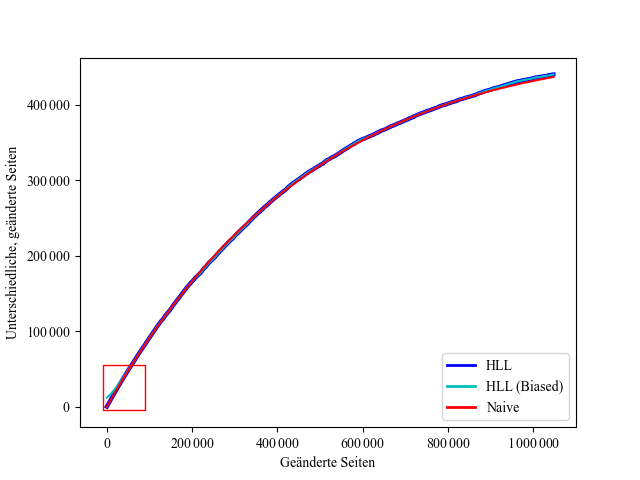
\includegraphics[width=.49\textwidth]{images/hll_count_1.png}
	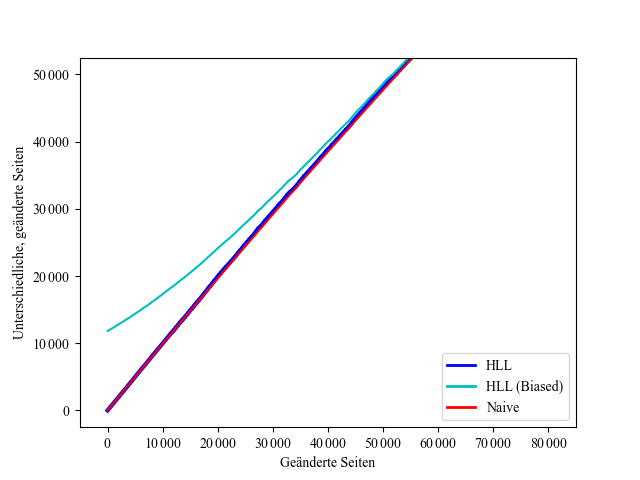
\includegraphics[width=.49\textwidth]{images/hll_count_2.png}
	\caption{Genauigkeit naiver Implementierung gegenüber HyperLogLog}
	\label{fig:hll-count}
\end{figure*}

Zum Testen eines approximativen Algorithmus haben wir uns für das Zählen unterschiedlicher Elemente mithilfe des HyperLogLog-Algorithmus entschieden.
Als Datenquelle haben wir die Änderungen von Wikipedia-Artikeln gewählt, um so zu approximieren, wie viele unterschiedliche Artikel täglich geändert werden.

Die Wikimedia Foundation bietet EventStreams für diverse Änderungen an.
Für unser Beispiel wichtig ist der unter https://stream.wikimedia.org/v2/stream/recentchange gelieferte Stream über alle Seitenänderungen.
Da der Stream Änderungen an diversen Wikis der Wikimedia Foundation überträgt, wurden die einkommenden Events nach der Domain ,,wikipedia.org`` gefiltert.

Die Seitennamen der eingehenden Events wurden dann auf drei verschiedene Arten gespeichert:  in einer Menge, um so eine naive Implementierung und einen Vergleichswert mit den Alternativen herzustellen, in einer bestehenden Implementierung des HyperLogLog-Algorithmus aus der gleichnamigen Python-Bibliothek \cite{evseenko2018} und in einer minimalen, eigenen Implementierung des Algorithmus, zu sehen im Anhang in \autoref{lst:hyperloglog}.
Die Genauigkeit des HyperLogLog-Algorithmus kann dabei proportional zum Speicherplatzbedarf gesteigert werden.
Dies erlaubt eine variable Genauigkeit.
Bei beiden verwendeten Algorithmen wurde deshalb eine maximale Abweichung von 1\% erlaubt.

Der Stream wurde über einen Zeitraum von 24~Stunden beobachtet und die Daten mitgeschrieben.
Anschließend wurden Informationen zum Speicherverbrauch und der Genauigkeit der beiden HyperLogLog-Implementierungen analysiert.

\subsection{Funktionsweise und Implementierung}

Beim HyperLogLog-Algorithmus werden eingehende Daten mit einer Hash-Funktion in eine zufällige Reihe aus Bits $\{0, 1\}^\infty$ umgewandelt.
Abhängig von der gewünschten Genauigkeit wird dann eine bestimmte Anzahl $b$ Bits weggenommen.
Diese Bits ergeben die binäre Speicheradresse eines Registers.
Dies führt zu $m=2^b$ unterschiedlichen Registern.
Je höher diese Zahl ist, desto genauer wird die Schätzung des Algorithmus.
Von den übrig bleibenden Bits des Hashes wird die Position von links des höchstwertigen 1-Bit bestimmt und in das entsprechende Register geschrieben.
Sollte das Register bereits einen höheren Wert enthalten, wird der alte Wert beibehalten.
Aus diesen Registern wird bei Abfrage ein stochastischer Erwartungswert berechnet, welcher der Anzahl unterschiedlicher, eingefügter Elemente entsprechen soll.
\cite{flajolet2007}

%\begin{equation}
%	\frac{n}{\frac{1}{x_1}+\frac{1}{x_2}+\ldots+\frac{1}{x_3}}=\frac{n}{\displaystyle\sum_{i=1}^{n}\frac{1}{x_i}}=\left(\frac{\displaystyle\sum_{i=1}^{n}x_i^{-1}}{n}\right)^{-1}
%	\label{eq:harmonic-mean}
%\end{equation}

Für den Algorithmus berechnet sich eine Abweichung abhängig von der Anzahl der Register $e=1.04/\sqrt{m}$ \cite{flajolet2007}.
Somit kann im Umkehrschluss auch die benötigte Anzahl an Registern und führenden Bits -- und somit auch der Speicherplatzbedarf -- aus einer gegebenen maximalen Abweichung wie in Gleichung~\eqref{eq:target-error} dargestellt berechnen.
In unserem Beispielprogramm benötigt die gewählte Genauigkeit von einem Prozent $b = log_2 (\frac{1.04}{0.01})^2 = 13.40$, beziehungsweise aufgerundet 14 führende Bits des Hashes.
Dies führt zu $m = 2^{14} = 16\,384$ benötigten Registern und somit einem maximalen Speicherverbrauch von 16\,384~Byte.

\begin{equation}
	\begin{alignedat}{2}
		& e & \: = \: & \frac{1.04}{\sqrt{m}} \\
		\Rightarrow \: & m & \: = \: & \left(\frac{1.04}{e}\right)^2 = 2^b \\
		\Rightarrow \: & b & \: = \: & \log_2 m = \log_2 \left(\frac{1.04}{e}\right)^2
	\end{alignedat}
	\label{eq:target-error}
\end{equation}

Bei der Beobachtung ergab sich im Bereich bis etwa 50\,000 einzigartiger Einträge eine starke Abweichung des selbst implementierten HyperLogLog-Algorithmus ohne Beachtung des Bias.
So erreichte dieser die gewünschte Genauigkeit von 99\% erstmals bei 49\,265 Einträgen und hielt sie konstant erst ab 49\,932.
Die Implementierung des HyperLogLog von \cite{evseenko2018} überschritt die Abweichung von 1\% über den gesamten Verlauf nur 356 mal.

Der gemessene Speicherbedarf bei der HyperLogLog-Implementierung lag, wie in \autoref{fig:hll-memory} dargestellt, stabil bei den zuvor berechneten 16\,384~Byte.
Demhingegen steigt der Speicherverbrauch der naiven Python-Implementierung in einer Menge rasant an.
Zu beachten ist hierbei die logarithmische Skala der Abbildung.
So steigt der Speicherbedarf des Python-Sets schon beim Einfügen des 309.
Elements auf das Doppelte des HyperLogLog-Speicherbedarfs und bis zum Ende auf das Zehnfache.

%\begin{figure}[h!]
%	\centering
%	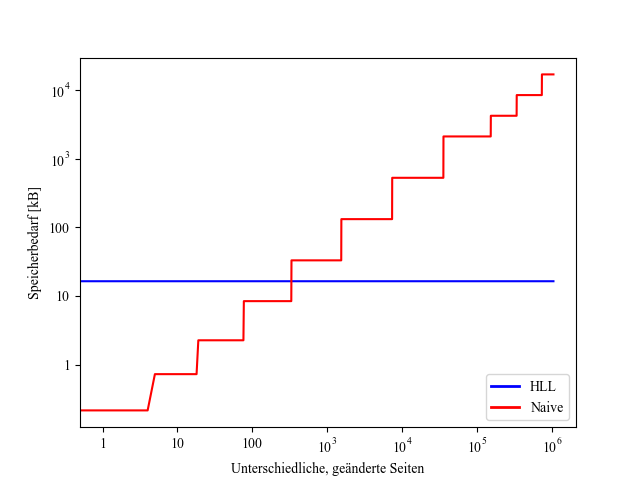
\includegraphics[width=0.49\textwidth]{images/hll_memory.png}
%	\caption{Speicherbedarf naiver Implementierung gegenüber HyperLogLog}
%	\label{fig:hll-memory}
%\end{figure}